% ==============================================================
\section{実験}\label{sec:experiments}
% ==============================================================

提案手法の有効性とスケーラビリティを検証する。
全実験はRust（リリースビルド）で実装し、
Apple M3（8コア、24\,GB RAM）上で実行した。

% ==============================================================
\subsection{EX-1：既存手法による密集領域の近似可能性}
\label{sec:ex1}\label{sec:ex1_1}
% ==============================================================

\paragraph{目的.}
\S\ref{sec:dense_detection}で定義した密集領域は
定義から一意に定まる厳密解であり、
提案手法はそれを計算する手段である。
本実験は提案手法と既存手法の精度競争ではなく、
既存手法がこの厳密解をどの程度近似できるかを評価し、
専用手法の必要性を検証するものである。

\paragraph{データ.}
4つの実データセットを使用した
（詳細はAppendix~\ref{sec:dataset_details}）。
Chicago Crime~\cite{chicagocrime}および
NYPD Crime~\cite{nypdcrime}は都市犯罪ドメイン、
NYC 311~\cite{nyc311}は市民苦情ドメイン、
USGS Earthquake~\cite{usgseq}は自然科学ドメインを代表し、
問題設定のドメイン横断的な汎用性を示す。
各データセットの生データは1イベントにつき1アイテム
（犯罪種別、苦情種別等）を含む。
連続座標（緯度、経度等）を等幅ビンに離散化してグリッドを構成し、
同一セルに属するイベントのアイテムを
1つのトランザクションに集約した
（1セル＝複数アイテムからなる1トランザクション；
グリッド構成の詳細はAppendix~\ref{sec:dataset_details}）。

\paragraph{比較手法.}
以下の手法を比較した。
パターンマイニング手法（Colocation / STCP-Miner）は
EX-1-1（密集パターン比較）のみに参加する。
領域抽出手法（MZoom / LISA / ST-DBSCAN）は
EX-1-2（密集領域比較）のみに参加し、
GTパターンを入力として与える。

\begin{itemize}
\item \textbf{Colocation}~\cite{shekhar2001colocation}: 空間コロケーションマイニング。PI閾値$\tau$をグリッドサーチ。
\item \textbf{STCP-Miner}~\cite{qian2009stcolocation}: Colocationの時空間ウィンドウ拡張。$\tau$およびウィンドウ幅をグリッドサーチ。
\item \textbf{MZoom}~\cite{shin2018mzoom}: GTパターン$P$の$d$次元出現テンソルに対する貪欲密集ブロック検出。Top $k$をグリッドサーチ。
\item \textbf{LISA}~\cite{anselin1995lisa}: GTパターン$P$の出現回数を空間グリッド上に集約し、Local Moran's $I$でHigh-Highセルを特定。
\item \textbf{ST-DBSCAN}~\cite{birant2007stdbscan}: GTパターン$P$の$d$次元出現セルに対し$\varepsilon_1$、$\varepsilon_2$、min\_ptsをグリッドサーチ。
\end{itemize}

\noindent 各比較手法のパラメータはグリッドサーチにより決定した
（詳細はAppendix~\ref{sec:grid_search_params_r1}）。
パターンマイニング手法はF1を最大化し、
領域抽出手法は平均Jaccardを最大化する設定を採用した。

\paragraph{評価指標.}
定義3--5に基づき、厳密パターン集合$P^*$および密集セル集合$R^*(P)$をGTとする。
パターンマイニング手法はF1
$= 2|\hat{P} \cap P^*| / (|\hat{P}| + |P^*|)$で評価し、
領域抽出手法はGTパターンを与えた上で
平均Jaccard $= \frac{1}{|P^*|}\sum_{P \in P^*} |R^*(P) \cap \hat{R}(P)| / |R^*(P) \cup \hat{R}(P)|$で評価する。

\paragraph{提案手法のパラメータ.}
全データセット共通：
時間ウィンドウ$W_0 = 53$（54週$\approx$1年）、
空間軸$W_k = 4$（5ビン、$k \geq 1$）。
閾値$\theta$はデータセットごとに
抽出パターン数が数十程度となるよう調整した
（Chicago: $\theta = 1{,}000$、NYPD: $\theta = 1{,}500$、
NYC 311: $\theta = 3{,}000$、USGS EQ: $\theta = 10$）。
最大パターン長は$|P| \leq 3$とした。

\paragraph{結果.}
Figure~\ref{fig:ex1_heatmap}に最良パラメータでの結果を示す。

\begin{figure}[t]
\centering
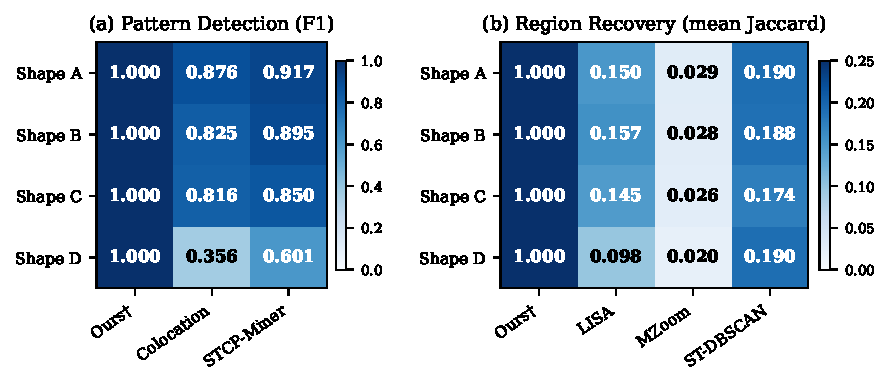
\includegraphics[width=\columnwidth]{fig/fig_ex1_heatmap.pdf}
\caption{EX-1の結果。
(a) パターン検出精度（F1）：パターンマイニング手法の最良パラメータでの結果。
(b) 領域復元精度（平均Jaccard）：GTパターンを与えた領域抽出手法の最良パラメータでの結果。
GTは定義3--5に基づく厳密解である。}
\label{fig:ex1_heatmap}
\end{figure}

\paragraph{分析.}
\emph{パターン検出精度（F1）。}
ColocationのグローバルPIは希釈の影響を受け、F1は0.26--0.69にとどまる。
STCP-Minerは時間ウィンドウにより改善するが、F1 $\leq$ 0.71に留まる。
いずれの手法も密集領域を出力しない。

\emph{領域復元精度（平均Jaccard）。}
MZoomは0.008--0.104、LISAは0.005--0.029、ST-DBSCANは0.007--0.027であり、
全データセットで0.11を下回る。
これは各手法の密度定義
（直積ブロック、時間集約、点近傍密度）が
スライディングウィンドウに基づく定義と構造的に異なるためである。
4次元データ（USGS EQ）でも同様の傾向が確認された。

% ==============================================================
\subsection{EX-2：スケーラビリティ（合成データ）}
\label{sec:ex2}
% ==============================================================

\paragraph{目的.}
提案手法の計算時間がトランザクション数$N$の増加に対して
どのようにスケールするか、
また同一$N$において時間軸長$T$と空間幅$s$の比率が
性能に影響するかを検証する。

\paragraph{合成データ生成.}
$d = 2$の格子
$\{0,\ldots,T{-}1\} \times \{0,\ldots,s{-}1\}$上で、
各アイテムを全セルに対して独立に
Bernoulli$(p_{\mathrm{item}}{=}0.10)$からサンプリングし、
1バスケットを構成する。
空セルにはデフォルトでアイテム1を割り当て、
各セルに正確に1トランザクションが存在することを保証するため、
$N = T \times s$となる
（生成の詳細はAppendix~\ref{sec:ex2_data_details}）。
$|\mathcal{I}| = 20$、$W = (24, 4)$、$\theta = 15$を固定した。

\paragraph{実験軸の選定根拠.}
$|\mathcal{I}|$および$p_{\mathrm{item}}$に対する線形スケーリングは
1次元版~\cite{aprioriwindow}で確認済みであり、
$d$の影響は$N = T \times s^{d-1}$に吸収される。
そのため$d = 2$を固定し、$T$と$s$の制御により$N$スケーラビリティを検証する。

\paragraph{実験設計.}
$T \in \{100,\; 1{,}000,\; 10{,}000,\; 100{,}000\}$および
$s \in \{10,\; 100,\; 1{,}000,\; 10{,}000\}$
の$4 \times 4 = 16$構成とした。
$N = T \times s$は$1{,}000$（$T{=}100, s{=}10$）から
$10^9$（$T{=}100{,}000, s{=}10{,}000$）の範囲をカバーする。
同一$N$で$T/s$比率が異なる構成が含まれるため、
時間軸長と空間幅が性能に与える影響を独立に観察できる。

\paragraph{結果.}
Table~\ref{tab:ex2_grid}に実行時間を示す。

\paragraph{分析.}
$N = 10^3$で0.009秒、$N = 10^8$で587--643秒であり、
$N$の$10^5$倍の増加に対して
実行時間の増加は約$6.5 \times 10^4$倍にとどまる。
$N = 10^9$は1{,}000秒以内に完了しなかった（タイムアウト）。

同一$N$でも$T/s$比率により差異が生じる：
$N = 10^7$において$T{=}100{,}000, s{=}100$は53.1\,sであるのに対し、
$T{=}1{,}000, s{=}10{,}000$は64.9\,s（1.22倍）である。
$T$が大きいほど$t$軸ストライド（Lemma~\ref{lem:stride}）による
ギャップスキップが有効に働き、
$s$が大きいほど空間始点数が増加するためである。

全体として実行時間は$N$に対しておおむね線形にスケールし、
$10^8$トランザクションを10分以内に処理可能である。

\begin{table}[t]
\centering
\caption{EX-2：2Dスケーラビリティ。
  全セルBernoulli背景のみ（埋め込みパターンなし）、
  $N = T \times s$、$\theta = 15$、$W = (24, 4)$。
  実行時間（秒）。$N = 10^9$は1{,}000\,s以内に完了せず。}
\label{tab:ex2_grid}
\small
\begin{tabular}{r|rrrr}
\toprule
$T \backslash s$ & 10 & 100 & 1{,}000 & 10{,}000 \\
\midrule
      100 & 0.009 &  0.059 &  0.655 &  7.18 \\
  1{,}000 &  0.042 &  0.470 &  5.62 &  64.9 \\
 10{,}000 &  0.403 &  4.79 &  57.5 &  643 \\
100{,}000 &  4.16 &  53.1 &  587 &     $>$1000 \\
\bottomrule
\end{tabular}
\end{table}
